\documentclass[a4paper]{article}

%% Language and font encodings
\usepackage[english]{babel}
\usepackage[T1]{fontenc}
\usepackage[utf8]{inputenc}
\usepackage{lipsum}
\usepackage{amsfonts}
\usepackage{graphicx} % Allows including images
\usepackage{booktabs} %
%% Sets page size and margins
\usepackage{listings}
\usepackage[most]{tcolorbox}
\usepackage{inconsolata}

%% Useful packages
\usepackage{amsmath}
\usepackage{graphicx}
\usepackage[colorinlistoftodos]{todonotes}
\usepackage[colorlinks=true, allcolors=blue]{hyperref}
\usepackage{amsfonts}
\usepackage{float}

\newtcblisting[auto counter]{sexylisting}[2][]{sharp corners, 
    fonttitle=\bfseries, colframe=gray, listing only, 
    listing options={basicstyle=\ttfamily,language=java}, 
    title=Listing \thetcbcounter: #2, #1}

\title{Uso de K-medias para el análisis de tránsito vehícular de la ciudad de Oporto\\ FES Acatlán,UNAM}
\author{César Armando Rojas Flores 	\\
Fernando Olvera Pérez }



\begin{document}
\maketitle
\newpage

\tableofcontents


\newpage

\section{Objetivo}

Realizar un análisis espacio temporal del tránsito vehícular por medio de clusters de la ciudad de Oporto, Portugal con dos finalidades:
\vspace{5mm}
\begin{itemize}
\item Mejorar la estimación de las tarifas base cobradas por la empresa de taxis que donó los datos.
\vspace{3mm}
\item Servir como insumo para la creación y mejora  políticas de publicas en cuestiones ambientales y de movilidad.
\end{itemize}

\section{Introducci\'on}
\begin{quote}
\textit{"Muy cerca del Atlántico, Oporto se levanta sobre la orilla derecha del Douro. Río arriba se extienden, sobre suelo esquistoso, los célebres viñedos.La ciudad a relieve accidentado se extiende hasta la orilla misma del Douro. Alrededor de la catedral (s.XII) centro medieval de la ciudad y su punto más elevado, la trama urbana es estrecha, pero une de cualquier forma las calles angostas y sinuosas a las rectilíneas del Renacimiento, además se abre a los jardines, parques y plazas urbanas como la Praça da Liberdade, al centro de Porto..."}\\
\vspace{10mm}
\textbf{Organización de las Ciudades Patrimonio Mundial.}
\end{quote}

\noindent
La ciudad de Oporto, Portugal con las coordenadas geográficas $41^{\circ}09'N 8^{\circ}36'O$  cuenta con una extensión geográfica de 41,42 $km^2$ una población censada en 2011 de 237,591, lo cual la convierte con casi la mitad de extención territorial de Lisboa en la segunda ciudad m\'as densamente poblada (\textit{hab}/$km^2$) de Portugal. Como muchas ciudades europeas debido a su antigüedad el trazado urbano no es optimo, lo que resulta en problemas de tr\'ansito vehícular, problemas de movilidad (transporte p\'ublico ) y mayor emisión de contaminantes, de aquí nace la motivación del trabajo.\\

\noindent
En Oporto convergen varias carreteras y líneas de ferrocarril, las cuales convierten a la ciudad en el principal centro comercial de toda la región norteña de Portugal. A pesar de la progresiva terciarizaci\'n del centro, la actividad industrial continúa siendo de gran importancia gracias a su cinturón industrial, que alberga fábricas de textiles, calzado, muebles, cerámica, metalurgia, orfebrería y otras actividades fabriles, además de algunas artesanales. Lo anterior implica necesariamente que exista un importante desplazamiento de capital humano, imperante para el desarrollo de las actividades industriales de la ciudad.\\

\noindent
Cabe resaltar que los datos no pertenecen exclusivamente a la ciudad de Oporto sino mas bien de la bien conocida Gran Área Metropolitana de Oporto, la cual cuenta con  17 municipios (concelhos) que, en el censo de 2001, contaban en total con 1.759.524 habitantes repartidos por una superficie de 2.038,88 $km^2$ y una densidad de 863 ($hab/km^2$). 

\section{Explicaci\'on del problema}
Como se mencionó dentro de la definición de objetivos, se busca realizar un an\'alisis del tr\'ansito vehícular por zona (cluster) y hora del día.\\

\noindent
El data set  utilizado en fue donado por una empresa de taxis, y recuperado de la plataforma Kaggle (\url{https://www.kaggle.com/crailtap/taxi-trajectory}), los taxis llevan un dispositivo de geo localizaci\'on (GPS). Los datos pertenecen 1,710,670 viajes de 448 taxis en el periodo de julio 2013 a junio 2014. Del data set se tomaron las siguientes variables:

\begin{itemize}
\item TRIP\_ID: (String) Identificador unico de cada viaje.
\item TAXI\_ID: (Integer) Identificador unico de cada taxi.
\item TIMESTAMP: (Integer) Timestamp de Unix (en segundos) asociado al inicio del viaje.
\item MISSING\_DATA: (Boolean) Bandera que indica cuando la información del GPS esta completa.
\item POLYLINE: (String) Contiene un lista de coordenadas de  GPS  con formato WGS84 mapeada como una cadena de texto. Cada par de coordenadas tiene la siguiente forma (LONGITUDE, LATITUDE). La lista contiene un par de coordenadas cada 15 segundos del viaje. A continuación una imagen que ejemplifica la estructura de las coordenadas: 
\begin{center}
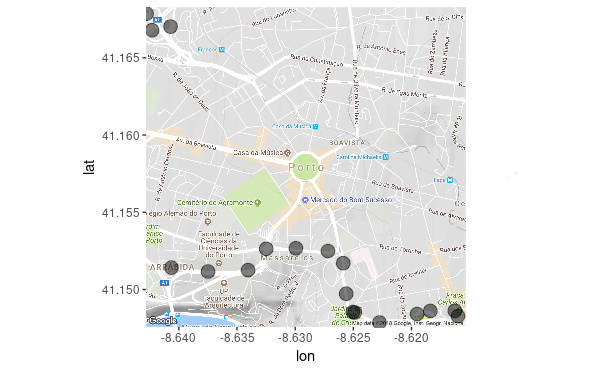
\includegraphics[width=0.9\textwidth]{mapa3.png}
\end{center}

\end{itemize}

\noindent
Se cuenta con m\'as datos de los que es posible analizar por lo cual se toma la decisión de eliminar, utilizando la variable MISSING\_DATA, los viajes que tienen alguna coordenada faltante, debido a la naturaleza de los datos, estos podrían ser interpolados pero el manejo se volvería m\'as complejo, los 1,710,670 viajes previamente reportados son obtenidos después de hacer el filtro con la bandera mencionada.\\

\noindent
Para el an\'alisis de la congesti\'n por zona (cluster) y tiempo (hora) es necesario tranformar el string POLYLINE utilizando la seccion de scripts 8.1, de tal forma que se puedan tener información puntual de las coordenadas pero que sea posible identificar la trayectoria y la hora del d\'ia, por lo que se crearon tres variables adicionales ,es importante aclarar que dicho tratameinto se da por chunks( trozos de observaciones del data set original) y se guarda en 171 archivos (\textit{all\_coordinates\_i.csv}) que contienen 83,408,417 observaciones y ocupan un espacio en memoria de aproximadamente 7Gb, con las siguientes variables adicionales:\\


\begin{itemize}
\item TRAY\_ID: (Integer) identifica la trayectoria ya que es necesario para el cálculo de la velocidad que las coordenadas sean adyacentes, ya que al hacer grupos geográficos se pueden perder, es decir, no todas caer al mismo cluster, por lo cual no se podrían utilizar para la velocidad promedio de cluster.

\begin{center}
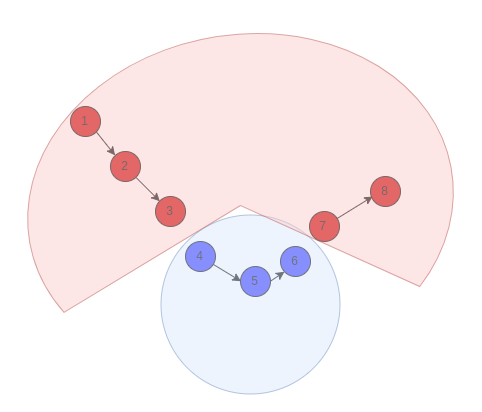
\includegraphics[width=0.6\textwidth]{trayectoria.png}
\end{center}

En el diagrama anterior se identifica lo descrito, la estimaci\'on de la velocidad ser\'a un promedio de la velocidad entre dos coordenadas adyacentes dentro de un mismo cluster, es decir la velocidad definida entre el nodo 4 y 5 se promediara con la del nodo 5 y 6 y sera asignada al cluster azul, para el cluster en rojo el razonamiento es el mismo. De lo anterior observamos dos cosas: a pesar que los nodos pertenecen a una misma trayectoria debido a los cluster geogr\'aficos, sus velocidades no son consideradas en el mismo grupo y que la velocidad del cluster es un promedio de la velocidad entre dos nodos adyacentes.
\item START\_FLAG: (boolean) Bandera que indica si la coordenada representa el inicio de un viaje, esta variable tiene la intención de obtener un conteo rápido de los viajes que comienzan por hora por cluster, por ejemplo.
\item END\_FLAG: (boolean) Bandera que indica si la coordenada representa el final de un viaje, esta variable tiene la intención de obtener un conteo rápido de los viajes que terminan por hora por cluster, por ejemplo. 
\end{itemize}

\noindent
Adicional, se transformo la variable TIMESTAMP para que tuviera informaci\'on temporal directamente relacionada con el punto en la trayectoria, con el fin de tener un promedio por hora mas preciso, es decir: \\

\begin{center}
TIMESTAMP = TIMESTAMP + (15*TRAY\_ID) 
\end{center}









\section{K-medias}
K-means es un método para encontrar clusters y centros de clusters en un conjunto de datos no
etiquetados, se inicia con un número definido de clusters sea k, y k-mean procede iterativamente
moviendo los centros de estos para minimizar el total de varianza de estos clusters el algoritmo
tiene dos pasos principalmente:
\begin{itemize}
\item Por cada centro identificamos el conjunto de datos de entrenamiento que están más cercanos a este.
\item La media de cada variable para el conjunto de puntos en cada cluster es calculada, y este vector de medias es el nuevo centro para ese cluster.
\end{itemize}

Como criterio de cercanía de los datos se usan medidas de proximidad, para medidas de proximidad tenemos las siguiente definici\'on.

\subsection{Medidas de proximidad}
Sean $X_{1},......,X_{p}$ variables y,
\\
$A=(a_{1},...,a_{p})$ valores de $X_{1},......,X_{p}$ para el individuo A
\\
$B=(b_{1},...,b_{p})$ valores de $X_{1},......,X_{p}$ para el individuo B
\\
Las proximidades son:

$$ disimilaridades : \delta(A,B) \rightarrow Distancias : d(A,B)$$
\\
$$ similaridades : \delta(A,B) \rightarrow Similitudes : s(A,B)$$
\\
\textbf{Distancia}: Una distancia es una aplicaci\'on  $d: \mathrm{R}^{p} X \mathrm{R}^{p} \rightarrow \mathrm{R}$ que verifica:
\begin{itemize}
\item $d(A,B)=0 \Longleftrightarrow A = B$
\item $d(A,B) + d(C,B) \geq d(A,C)$
\end{itemize}
La distancia mide lo lejano que están dos puntos.
\textbf{Similitud}: una similitud es una aplicaci\'on $s: \mathrm{R}^{p} X \mathrm{R}^{p} \rightarrow \mathrm{R}$ que verifica :
\begin{itemize}
\item $0 \leq s(A,B) \leq 1 \forall_{i,j}$.
\item $s(A,B) = 1 \Longleftarrow A = B$.
\item $s(A,B) = s(B,A)$.
\end{itemize}

\section{K-medias ++}
Kmedias++ es una variante de k-medias y esta tiene algunas ventajas y desventajas que son:
\\
\begin{itemize}
\item Gasta tiempo escogiendo los centros iniciales en cada iteraci\'on.
\item Ahorra tiempo en el agrupamiento o clustering.
\end{itemize}
k-means varia en cómo escoge los centroides, ya que escoge como centroides aquellos que estén m\'as lejos entre ellos, la explicaci\'on es la siguiente:
\\
Se escoge un centro de $X$ aleatoriamente
\begin{itemize}
\item Se escoge un centro de $X$ aleatoriamente.
\item Para $k-1$ veces.
\item ...Toma un centro de $X$ con probabilidad $p$.
\item ...Actualiza la matriz de centros.
\end{itemize}
\newpage
Ejemplo.
\\
\\
Como escoger $k$ centros.
\begin{center}
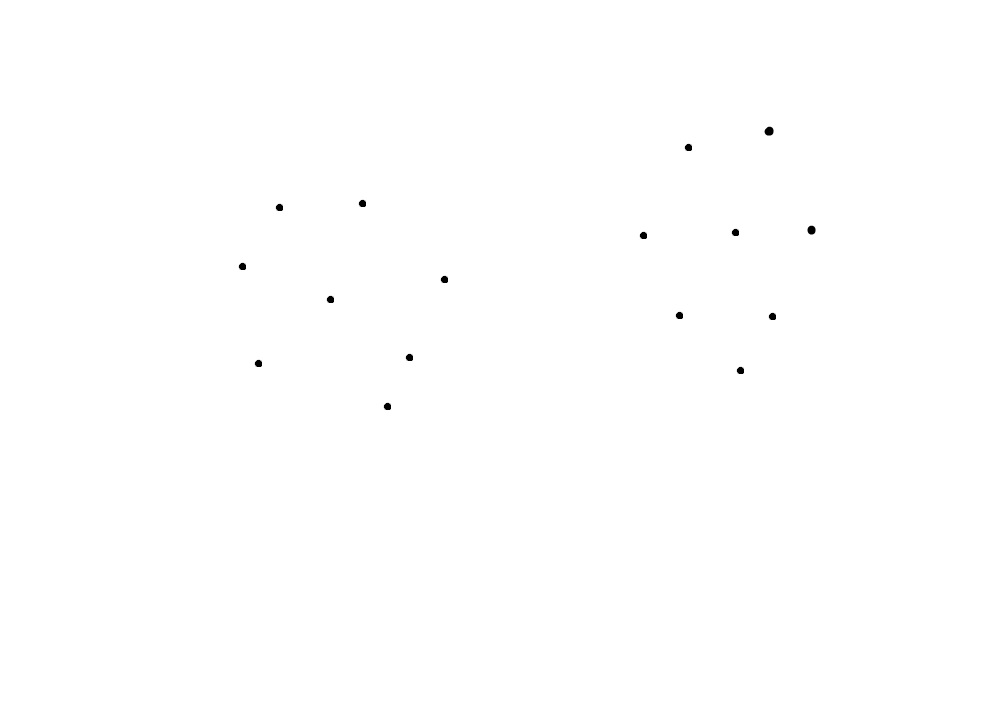
\includegraphics[width=0.9\textwidth]{puntos.png}
\end{center}
Escoge un punto de $X$ Aleatoriamente.
\begin{center}
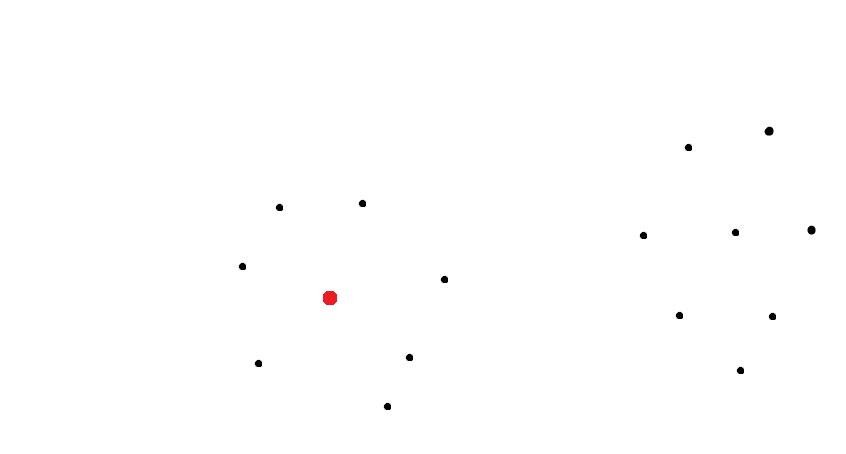
\includegraphics[width=0.7\textwidth]{puntos_aleatorios.png}
\end{center}
Calcula todas las $d_{i}^{2}$ donde $d_{i}^{2}=min(Distancia euclidiana a cada punto)$
\begin{center}
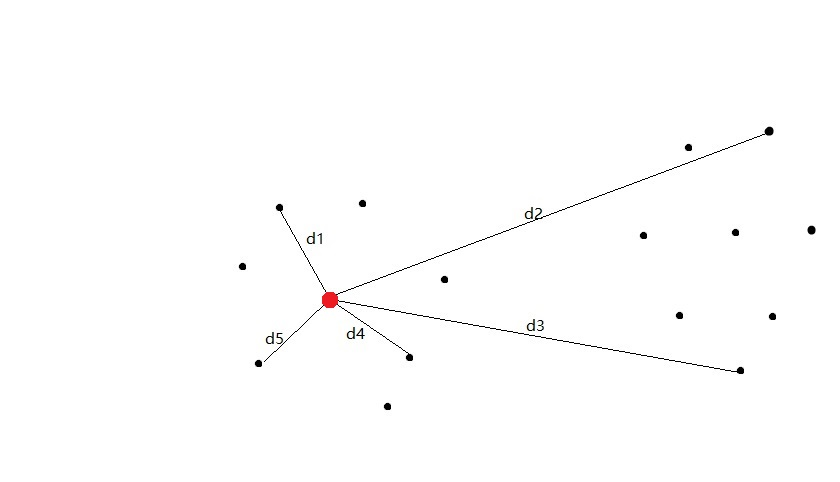
\includegraphics[width=0.7\textwidth]{all_distances.png}
\end{center}
\newpage
Calcula $P_{i}$
\begin{itemize}
\item $D=d_{1}^{2}+d_{2}^{2}+d_{3}^{2}+...+d_{n}^{2}$.
\item $P_{i}=d_{i}^{2}/D$.
\item $\sum P_{i} = 1$
\end{itemize}
Los puntos m\'as alejados de un centro tienen mayor probabilidad de ser escogidos.
\\
Tomamos otro punto con probabilidad $P$.
\begin{center}
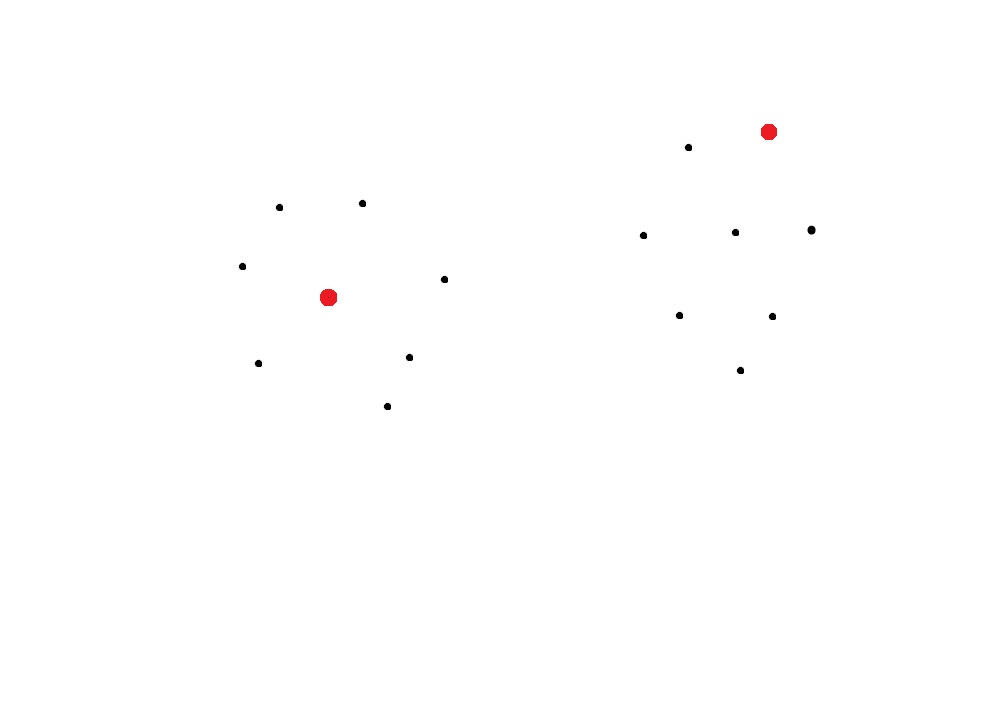
\includegraphics[width=0.7\textwidth]{tomar_otro_punto.png}
\end{center}
Despu\'es nos mantenemos:
\begin{itemize}
\item Actualizando la matrix de centros.
\item Calcular $d_{i}^{2}$.
\item Calular $P_{i}$.
\end{itemize}
Esto hasta que $k$ centros sean encontrados.
\\
Hay que destacar que despu\'es de la selecci\'on de puntos iniciales este algoritmo converge muy rapido.

\section{Resultados}

La complejidad del algoritmo original de K-medias es

\begin{displaymath}
O(n^{dk+1}log n)
\end{displaymath}
Donde 
\begin{displaymath}
O(g(n)) = \{ f: \mathbb{N} \to \mathbb{R}^+ | \exists c , n_o \epsilon \mathbb{N}:f(n)\leq cg(n), \forall n\geq n_0 \}
\end{displaymath}
La notación O representa una cota superior del numero de operaciones que se deben de hacer dependiendo de los parámetros del algoritmo, en este caso es exponencial, lo cual afecta el desempeño en tiempo y espacio, debido a esto  y coniderando $n=83,498,417$  y que la ciudad de Oporto cuenta con 17 municipios (concelhos) se optó por considerar a k=8, esto debido a que d=2 es decir estamos en un plano pero el problema aun  es NP Hard, aunado a que es el número de clusters es aproximademnete la mitad de municipios de la ciudad.\\


\noindent
La ejecución se hizo utilizando K-medias ++ en un servidor con 64 Gb de ram, y 16 cores de procesamiento y esta se hizo en R, Python y Spark, obteniendo la siguiente distribuci\'on de observaciones en cada cluster.\\

\noindent
Debido a la cantidad de datos para que sean visibles los grupos se muestra un chunk  (sección de 473,778 observaciones del archivo all\_coordinates\_100.csv) del data set original con los cluster resultantes al chunk:
\begin{figure}[H]
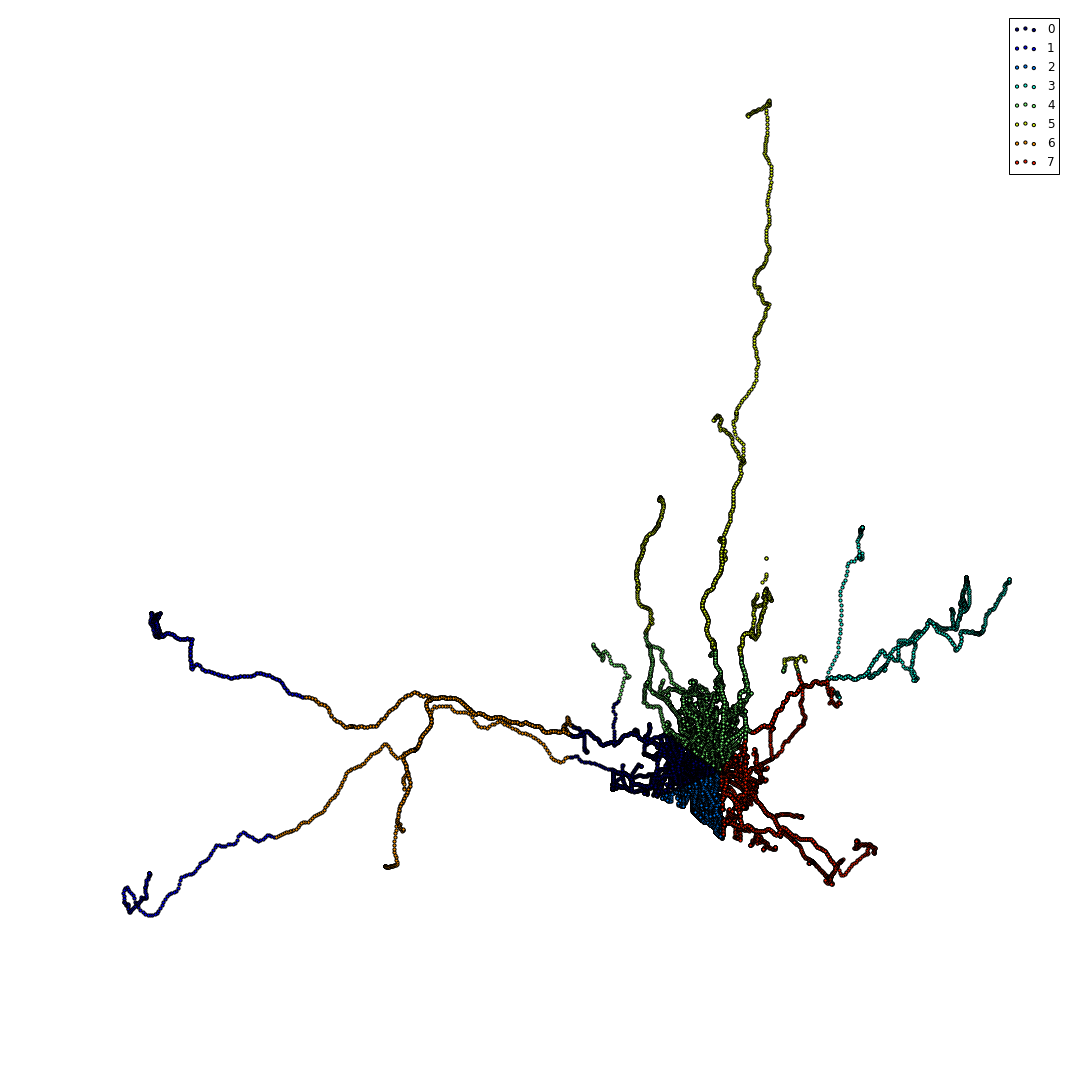
\includegraphics[scale=.3]{descarga_1.png}
\end{figure}

\noindent
Al estar las coordenadas determinadas por latitudes y longitudes se debería contemplar la curvatura de la tierra para el cálculo de distancias, al realizar k-medias se consideró a las longitudes y latitudes como puntos sobre un plano y se utilizó la distancia euclidiana, esto debido a que la proximidad de los puntos no se ve afectada por la curvatura de la tierra ni es necesario considerar una escala especifica, pero para las velocidades, necesitamos la distancia entre cada para de nodos adyacentes expresada en kilómetros, por lo que se usara la distancia de Haversine, descrita en la siguiente subsección.\\

\noindent



\subsection{Distancia de Haversine}
Dados dos puntos sobre una superficie esf\'erica el usar para c\'alculo de la distancia m\'etodos que no contemplan la curvatura de la superficie puede afectar un poco la medida obtenida mas si estos puntos estan muy alejados.
\\

\begin{center}
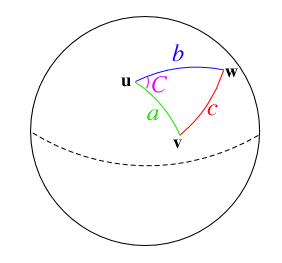
\includegraphics[width=0.7\textwidth]{haversine.png}
\end{center}
La funci\'on de haversine se define como:
\begin{displaymath}
haversine\left(\frac{d}{r}\right)=haversine\left(\phi_{2} - \phi_{1} \right) + cos(\phi_{1})cos(\phi_{2})haversine\left(\lambda_{2}-\lambda{1}\right)
\end{displaymath}
\begin{center}
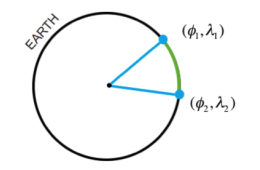
\includegraphics[width=0.4\textwidth]{haverseno.png}
\end{center}
Donde $haversine$ se define como:
\begin{displaymath}
haversin (\theta) = sen 2 (\frac{\theta}{2}) = (1-cos ( \theta ))/2
\end{displaymath}
De aqui podemos obtener la distancia, que esta definida como:
\begin{displaymath}
d=2rarcsin\left(\sqrt{sin^{2}\left(\frac{\phi_{2} - \phi_{1} }{2}\right)+ + cos(\phi_{1})cos(\phi_{2})sin^{2}\left(\frac{\lambda_{2} - \lambda_{1} }{2}\right)} \right)
\end{displaymath}
Donde $r$ es el radio de la tierra.
\subsection{Velocidad Promedio por Hora y por Cluster.}

Con la distancia en kilómetros estamos listos para estimar la velocidad por cluster por hora, para lo cual se puede observar en  la sección 8.2 los scripts que agrupan y estiman la velocidad, resumiendo se toma la distancia en kilometros y considerando que cada entre cada nodo hay 15 segundos, estimamos:

\begin{displaymath}
vel(km/h)  =  d(km) \left(15s\frac{1h}{3600s}\right)^{-1}
\end{displaymath}

\noindent
Con los grupos sobre los 83,498,417 millones de registros se estiman las siguientes velocidades por grupo:

\begin{center}
\begin{tabular}{crr}
\toprule
{} &  CLUSTER &  VELOCIDAD \\
\midrule
 &        1 &  63.827000 \\
 &        2 &  37.126140 \\
 &        3 &  59.160192 \\
 &        4 &  76.874780 \\
 &        5 &  72.853568 \\
 &        6 &  36.431142 \\
 &        7 &  26.113135 \\
 &        8 &  51.808664 \\
\bottomrule
\end{tabular}
\end{center}

\noindent
De la misma forma se estima la velocidad de los cluster por hora, con el fin de evaluar la velocidad y tener una definición espacio temporal del tránsito vehícular


\begin{center}
\begin{figure}[H]
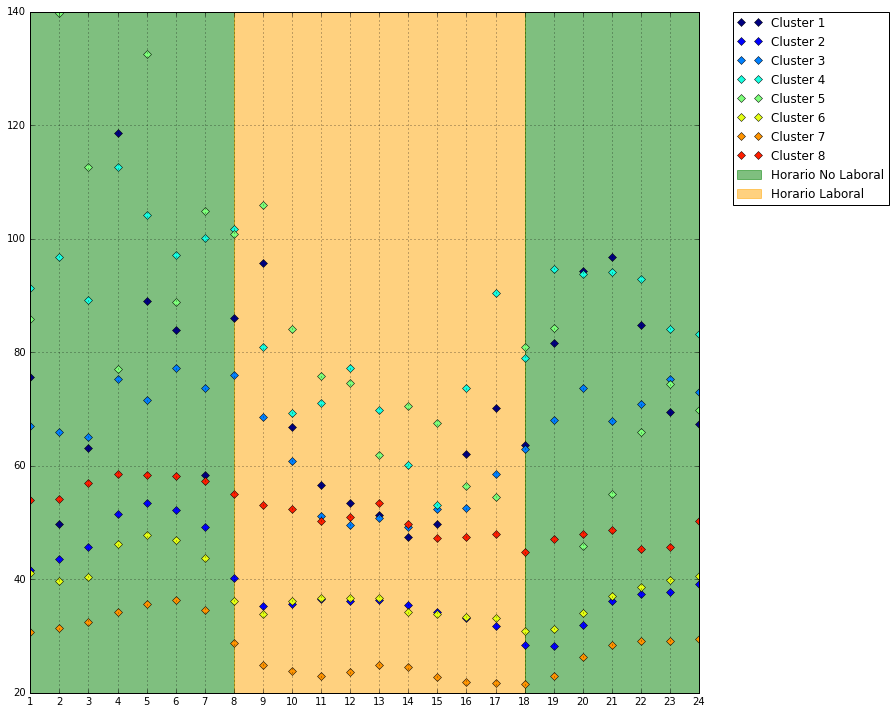
\includegraphics[scale=.4]{velperclus.png}
\end{figure}
\end{center}

\noindent
El gráfico anterior nos da indicios de como es el tránsito, por hora hay un bajón generalizado en todos los clusters durante la jornada laboral, a excepción de los que tienen velocidades promedio más grandes sucede en las primeras horas de la jornada laboral esto se puede explicar por que estas zonas están relativamente alejadas de la zona de mayor congestión, es decir los puntos se encuentran mas dispersas pero a medida que se acercan a una zona con tránsito denso bajan durante la jornada laboral. Se observa que solo el cluster siete mantiene velocidades por debajo de 40km/h a cualquier hora del día, esta información podría servir para establecer una tarifa base para los viajes que comienzan en ese cluster por encima de las demás zona geográficas.Lo mismo para los clusters dos,seis,siete y ocho los cuales en cualquier hora del día tienen velocidades menores a 60 km/h, la asignación de tarifas base por zona podría mejorar los ingresos de la empresa de taxis. Pero analicemos la cantidad de viajes que comienzan en cada cluster por hora:
\begin{center}
\begin{figure}[H]
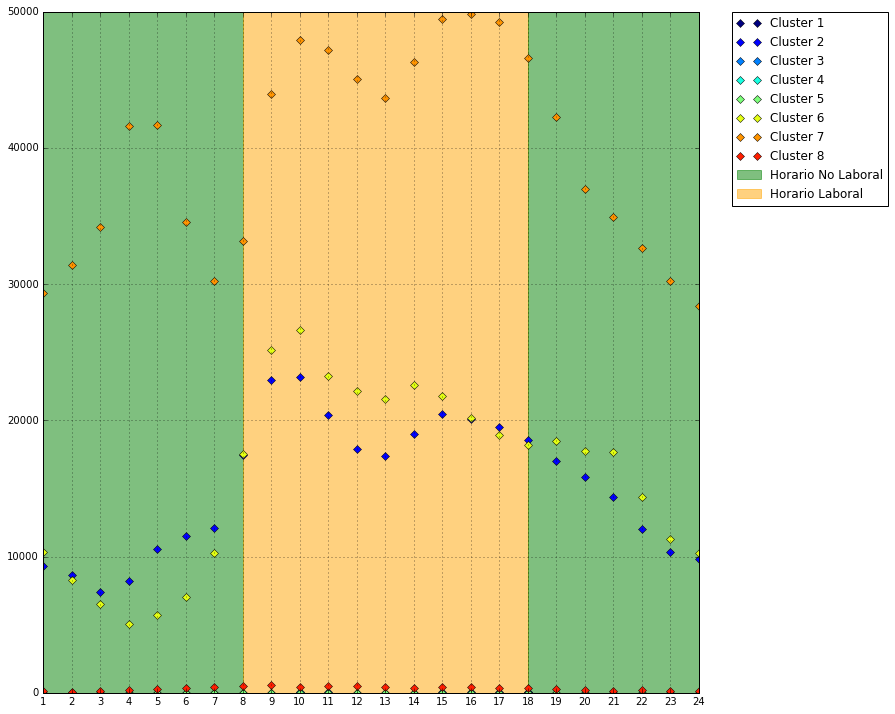
\includegraphics[scale=.4]{descarga_22.png}
\end{figure}
\end{center}
 
 \newpage
 \noindent
 Ahora veamos la cantidad de viajes que terminan por cluster por hora:
 \begin{center}
\begin{figure}[H]
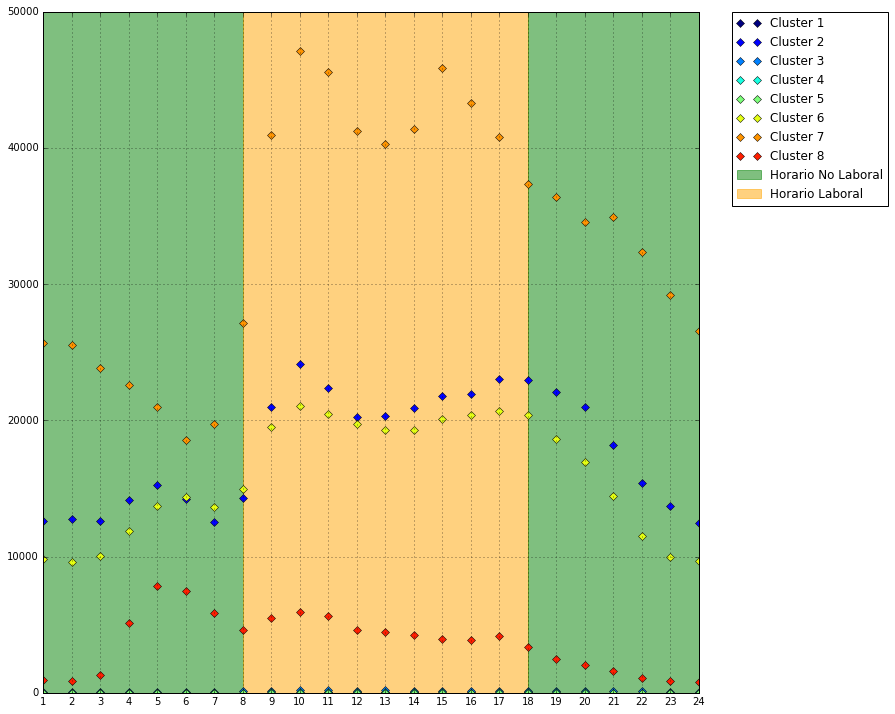
\includegraphics[scale=.4]{descarga_23.png}
\end{figure}
\end{center}

\noindent
De ambos gráficos podemos concluir que el cluster más denso es el siete, pero que durante las primeras horas del día comienzan mas viajes de los que terminan, esto nos da indicios de movilidad, y que en esas horas la tarifa base podría ser menor, esta clase de análisis le servirían a la empresas de taxis a captar una mayor cantidad de mercado ya que la estimación precisa, de la oferta y demanda por zona geográficas y horas del día. podría ayudar a cubrir una mayor cota de mercado, lo cual se traduce en más beneficios económicos.
\\
\\
\textbf{Nota:} Las gráficas mostradas fueron hechas con muestras de los resultados, ya que el dibujado de gráficos para todos los registros requiere mayor uso de recursos aun mayor que el usado para ejecutar k-medias
\section{Conclusiones}

Los clusters demostraron que la velocidad promedio que determina la congestión vehícular tiene una distribución heterogénea, es decir encontramos segmentos geográficos en donde la velocidad difiere considerablemente, esta información puede servir a la empresas de taxis a definir tarifas base por hora por zona geográfica, incluso  como trabajo posterior podrían diseñarse cierres convexos para las zona geográficas, asimismo el numero de viajes que terminan y comienzan por segmento por hora pueden ayudarnos como se menciono anteriormente a la optimización de la asignación de taxis por región geográfica por horario con el fin de maximizar las utilidades de la empresa.
Las políticas publicas en cuestiones de movilidad pueden considerar en donde comienzan y terminan mas viajes para determinar si se cuenta con un sistema de transporte publico eficiente, de igual forma las velocidades pueden servir para estimar las emisiones contaminantes y la creación de políticas publicas amigables con el medio ambiente, como medios de transporte alternativos.


\section{Scripts}
\begin{sexylisting}{Scrip 8.1}
chunksze   = 10000
count = 0
for chunk in 
pd.read_csv('train_womissings.csv', chunksize=chunksze):

count+=1
        file_name = "all_coordinates_"+str(count)+".csv"
        print (time.ctime())
        str_arr = np.array(chunk[['POLYLINE',
        'DAY_TYPE','TIMESTAMP','TAXI_ID','TRIP_ID']])
        def lambdaf(x):
            y=np.matrix(x[0])
            y=y.reshape(int(y.shape[1]/2),2)
            day_type = np.array(y.shape[0]*[ord(x[1])])
            timestamp = np.array(y.shape[0]*[x[2]])
            taxi_id = np.array(y.shape[0]*[x[3]])
            trip_id = np.array(y.shape[0]*[x[4]])
            trayectory_id = np.arange(y.shape[0])
            start_flag = np.zeros(y.shape[0])
            end_flag = np.zeros(y.shape[0])
            start_flag[0] = 1
            end_flag[y.shape[0]-1] = 1
            x = np.column_stack(
            (y,day_type,timestamp,
            taxi_id,trip_id,trayectory_id,start_flag 			  					,end_flag))
            return x
        all_coordinates = 
        np.concatenate([lambdaf(x) for x in str_arr])
        print (time.ctime())
        df=pd.DataFrame(all_coordinates,columns
        ['LATITUD','LONGITUD','DAY_TYPE','TIMESTAMP',                              'TAXI_ID','TRIP_ID','TRAYECTORY_ID',
        'START_FLAG','END_FLAG'])
        print (file_name +" *DONE* ")
        df.to_csv(file_name)

\end{sexylisting}
\subsection{K-meadias en python, R y spark}
\begin{sexylisting}{K-medias (python)}
kmeans = 
KMeans(n_clusters=8, random_state=0).
fit(df[['LONGITUD','LATITUD']])
df['CLUSTER']= kmeans.labels_
\end{sexylisting}
Para la ejecuci\'on en R se opto por ejecutar directamente el archivo en R desde consola ya que fue ejecutado en servidor con comando

\begin{sexylisting}{Ejecucion script de R}
R < Script.r --no-save
\end{sexylisting}


\begin{sexylisting}{Ejecucion script de R}
library(readr)
all_data_kmeans <- 
read_csv("/home/fernando/all_data_kmeans.csv")
grupos<-
kmeans(all_data_kmeans,8)
write.csv(grupos$cluster, 
file="/home/fernando/grupos.csv")
\end{sexylisting}

\begin{sexylisting}{K-means en scala con spark}
// 
// Input data: archivos delimitados por comas
// latitud (4 campo) y longitud (5 campo)


import scala.math.pow

// distancia entre dos puntos
def distanceSquared
(p1: (Double,Double), p2: (Double,Double)) = { 
  pow(p1._1 - p2._1,2) + pow(p1._2 - p2._2,2 )
}

// suma de dos puntos
def addPoints
(p1: (Double,Double), p2: (Double,Double)) = {
  (p1._1 + p2._1, p1._2 + p2._2)
}


//para un punto p en un array de puntos, 
//regresa el indice en el array mas cercano al punto p
def closestPoint(p: (Double,Double), points: 
Array[(Double,Double)]): Int = {
    var index = 0
    var bestIndex = 0
    var closest = Double.PositiveInfinity

    for (i <- 0 until points.length) {
      val dist = distanceSquared(p,points(i))
      if (dist < closest) {
        closest = dist
        bestIndex = i
      }
    }
    bestIndex
}

// Lectura de archivos
val filename = "/loudacre/all_coordenates/*"

// K es numero de centros a encontrar
val K = 8

// umbral de distancia entre cada centro 
//para saber cuando parar
val convergeDist = .01D
    
// parsea el archivo y lo corta por comas
// parsea latitud y longitud que son
//la cuarta y quinta columna
val puntos = sc.textFile(filename).
     map(line => line.split(',')).
     map(fields => 
     (fields(3).toDouble,fields(4).toDouble)).
     persist()


\end{sexylisting}

\begin{sexylisting}{K-means scala 2d parte}
//inicia con k centros elgidos aleatoriamento 
//del dataset
val kPoints = points.takeSample(false, K)
println("Starting K points:")
kPoints.foreach(println) 

// loop que termina hasta que 
//la distancia entre los puntos 
//y los centros converga o 
//no varia mucho en cada iteracion
var tempDist = Double.PositiveInfinity
while (tempDist > convergeDist) {


    val closest = 
    points.map(p => (closestPoint(p, kPoints), (p, 1)))

    val pointStats = 
    closest.reduceByKey{case ((point1,n1),(point2,n2)) 
    => (addPoints(point1,point2),n1+n2) }

    val newPoints = 
    pointStats.map{case (i,(point,n))
    => (i,(point._1/n,point._2/n))}.collectAsMap()
    

    tempDist = 0.0
    for (i <- 0 until K) {
      
      tempDist += distanceSquared(kPoints(i),
      newPoints(i))
    }
    println("distancia entre iteraciones: "+tempDist)

    for (i <- 0 until K) {
      kPoints(i) = newPoints(i)
    }
}
   
// desplieaga los centros finales       
println("Final K points: " )
kPoints.foreach(println)
\end{sexylisting}

\subsection{Agrupamientos y resultados}
Ya con los resultados ejecutamos scripts en python para obtener velocidades por hora, cluster y promedio de velocidad por cluster.
\\
\begin{sexylisting}{Obteniendo la hora y conteo de inicios de vaijes y finales por hora}
df = 
pd.read_csv('/home/All_coordenates/para_python2.csv')
df['HORA'] = df.TIMESTAMP.dt.hour
start = 
df.groupby(['cluster','HORA'])['START_FLAG'].sum()
end = 
df.groupby(['cluster','HORA'])['END_FLAG'].sum()
\end{sexylisting}
\begin{sexylisting}{Determinar trayectorias completas por cluster}
df['LAG_TRAYECTORY_ID'] =
df.groupby(['cluster','TRIP_ID'])['TRAYECTORY_ID'].
shift(1)

df = df.loc[(df.TRAYECTORY_ID-df.LAG_TRAYECTORY_ID)==1]
\end{sexylisting}
\begin{sexylisting}{Lags sobre las longitudes para poder cálcular distancias ya que se necesita sobre dos nodos adyacentes}
df['LAG_LONG'] = 
df.groupby(['cluster','TRIP_ID'])['LONGITUD'].shift(1)
df['LAG_LAT'] = 
df.groupby(['cluster','TRIP_ID'])['LATITUD'].shift(1)
\end{sexylisting}
\begin{sexylisting}{distancias de la trayectoría utilizando distancia esferica entre coordenadas}
def haversine_np(lon1, lat1, lon2, lat2):
    lon1, lat1, lon2, lat2 = 
    map(np.radians, [lon1, lat1, lon2, lat2])
    dlon = lon2 - lon1
    dlat = lat2 - lat1
    a = np.sin(dlat/2.0)**2 + 
    np.cos(lat1) * np.cos(lat2) * np.sin(dlon/2.0)**2
    c = 2 * np.arcsin(np.sqrt(a))
    km = 6367 * c
    return km
df['DISTANCIA'] = 
haversine_np(df.LAG_LONG, df.LAG_LAT,df.LONGITUD, df.LATITUD)
\end{sexylisting}

\begin{sexylisting}{velocidad en km/h distanciakm/15/3600}
df['VELOCIDAD'] =df['DISTANCIA']/0.00416666666
\end{sexylisting}

\begin{sexylisting}{velocidad promedio del cluster}
df.groupby(['cluster'])['VELOCIDAD'].mean()
\end{sexylisting}

\begin{sexylisting}{Promedio velocidad por hora}
to_plot=
df.groupby(['cluster','HORA'])['VELOCIDAD'].mean()
print(to_plot)
\end{sexylisting}
\newpage

\section{Recursos}

\section{Bibliografia}
\begin{itemize}
	\item "http://theory.stanford.edu/~sergei/papers/vldb12-kmpar.pdf",$(accessed: 02.05.2018)$
	\item "https://www.npmjs.com/package/haversine-geolocation",$(accessed: 02.05.2018)$
	\item "Mahil Herrera".II An\'alisis de Conglomerados,$(accessed: 02.05.2018)$
    \item "https://github.com/cloudera/spark/blob/master/mllib/src/main/scala/org/apache/spark/mllib/clustering/KMeans.scala",$(accessed: 02.05.2018)$
\end{itemize}





\end{document}